\section{Detector Overview}
\label{sec:detector-overview}

The PIONEER detector is organized around the stopped-pion target. The active
target sits at the beam focus and records the pion stop, possible intermediate
muon track, and outgoing charged particle topology. A low-mass tracking layer
outside the target may provide additional positron direction and matching
information. The surrounding electromagnetic calorimeter measures the
positron energy and time with high resolution. This layout follows directly
from the Phase-I \(R_{e/\mu}\) strategy: the calorimeter separates the
\(\pi\to e\nu\) energy peak from the Michel spectrum, while the inner
detectors classify the decay topology and constrain the correction factors
discussed in \secref{sec:measurement-strategy}.

\begin{figure}[!htbp]
  \centering
  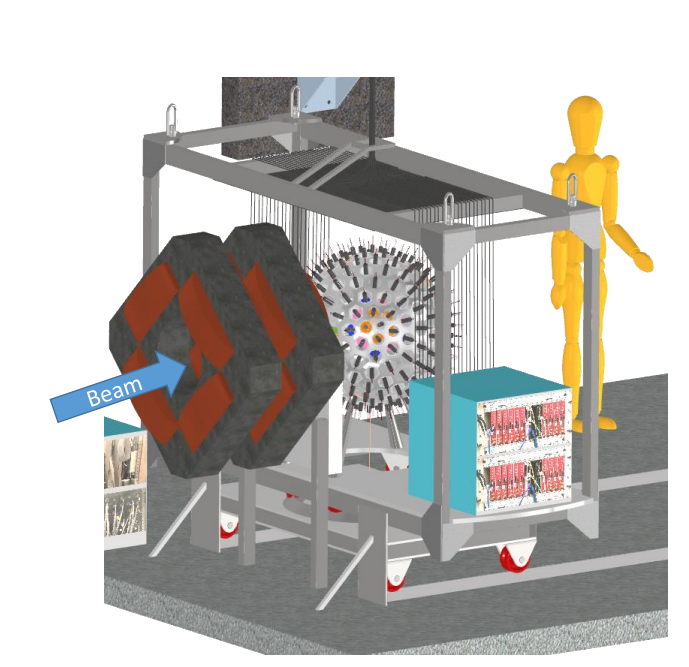
\includegraphics[width=0.50\textwidth]{../resources/figures/chapters/01_introduction/3d_detector_render}
  \caption{Conceptual rendering of the PIONEER detector layout. The ATAR and tracker are surrounded by a segemented LYSO calorimeter calorimeter.}
  \label{fig:pioneer-detector-render}
\end{figure}

\subsection{Calorimeter}
\label{subsec:detector-overview-calorimeter}

The calorimeter provides the primary measurement of the outgoing positron
energy. For Phase I, most of the discriminating information lies in the
\(\withunit{50}{\mega\electronvolt}\) to
\(\withunit{70}{\mega\electronvolt}\) range, where the Michel spectrum ends
and the direct \(\pi\to e\nu\) peak appears. The detector therefore needs
high energy resolution, high efficiency, fast timing, and enough depth and
angular coverage to minimize shower leakage. Segmentation and timing are also
needed to control pileup at the high stopped-pion rate. This is motivated in
part by the PIENU measurement, for which the low-energy response tail was a
dominant systematic limitation in the extraction of \(R_{e/\mu}\)
\cite{AguilarArevalo:2015cdf,pioneer_proposal_2022}. Current calorimeter
performance targets are set by simulations and include roughly
\(19X_{0}\) depth, fiducial polar coverage near
\(\withunit{120}{\degree}\), effective energy resolution near
\(\withunit{1.85}{\percent}\) at \(\withunit{70}{\mega\electronvolt}\) and
\(\withunit{2.2}{\percent}\) at \(\withunit{56}{\mega\electronvolt}\), timing
near \(\withunit{200}{\pico\second}\) at
\(\withunit{56}{\mega\electronvolt}\), and pulse-pair separation at the
\(\order{\withunit{10}{\nano\second}}\) scale
\cite{pioneer_proposal_2022,lyso_calo_intro_2025,tapered_lyso_pioneer_2026}.

This dissertation focuses on the lutetium-yttrium oxyorthosilicate (LYSO)
calorimeter program. LYSO is attractive because it is dense, fast, bright,
and radiation hard. Its dominant elemental constituents are lutetium,
oxygen, silicon, and yttrium, with a small cerium dopant that provides the
scintillation centers. Typical material parameters relevant here are a density
of \(\withunit{7.4}{\gram\per\centi\meter\cubed}\), radiation length
\(\withunit{1.14}{\centi\meter}\), Moliere radius
\(\withunit{2.07}{\centi\meter}\), scintillation decay time near
\(\withunit{40}{\nano\second}\), and light yield of order
\(\withunit{30000}{photons\per\mega\electronvolt}\)
\cite{beesley_lyso_threshold_2024,tapered_lyso_pioneer_2026}. The radiation
length sets the longitudinal shower-containment scale, while the Moliere
radius sets the transverse scale for electromagnetic shower spread. Together,
these properties allow a compact crystal calorimeter with fast response and
substantial intrinsic light output at the positron energies relevant for
PIONEER.

The current LYSO concept uses a quasi-spherical pointing geometry based on a
\((6,0)\) Goldberg polyhedron. In the full sphere this geometry contains 362
crystals; with the beam entrance region removed, the Phase-I calorimeter
contains 311 crystals. The crystal inventory consists of eight shapes: one
class of tapered pentagon and seven classes of tapered hexagon
\cite{tapered_lyso_pioneer_2026}. The pointing geometry is important because
it reduces inactive material at the front face and provides nearly complete
coverage around the target. The same geometry also defines several design
requirements: large tapered crystals must preserve longitudinal response
uniformity, be mounted from the rear, and keep inactive material between
crystals small.

\begin{figure}[!htbp]
  \centering
  \begin{subfigure}{0.42\textwidth}
    \centering
    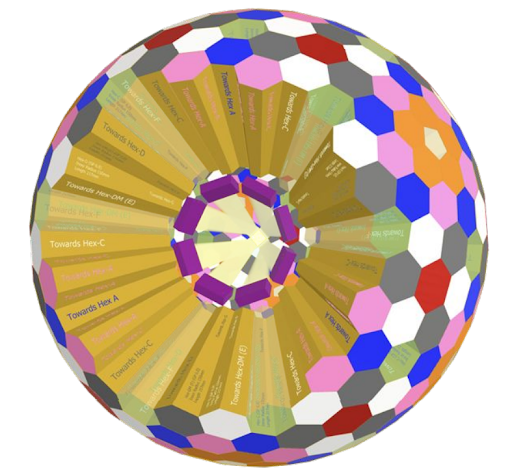
\includegraphics[width=\textwidth]{../resources/figures/chapters/01_introduction/lyso_goldberg}
    \caption{3D Render of full calorimeter based on (6,0) Goldberg polyhedron geometry}
  \end{subfigure}
  \hfill
  \begin{subfigure}{0.48\textwidth}
    \centering
    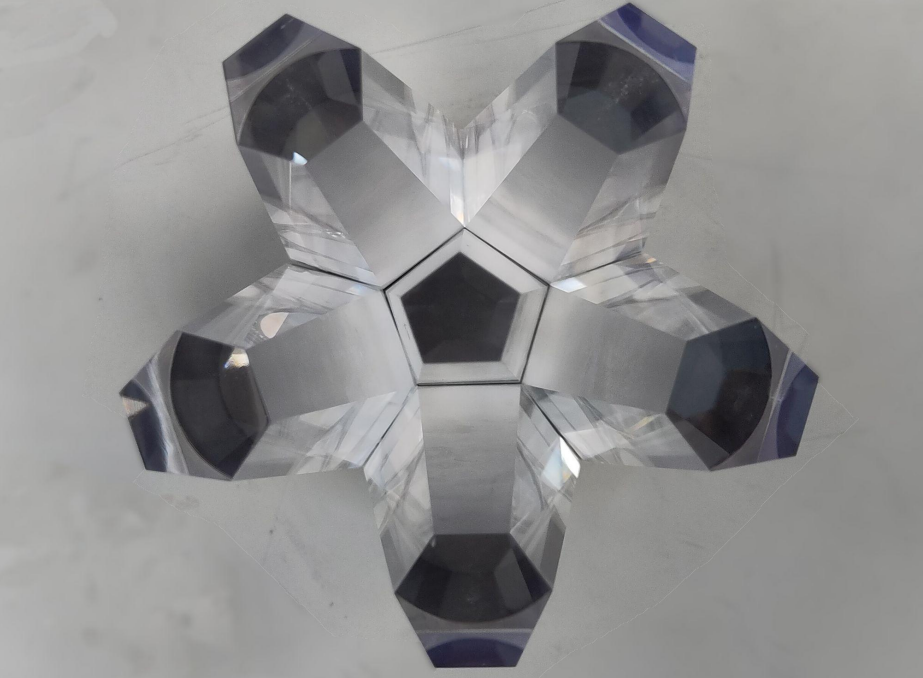
\includegraphics[width=\textwidth]{../resources/figures/chapters/01_introduction/LYSO_pent_segment}
    \caption{Goldberg polyhedron segment containing a pentagonal crystal}
  \end{subfigure}
  \caption{Pointing LYSO calorimeter geometry. The tapered pentagonal and
  hexagonal crystals provide a nearly gapless calorimeter surface while
  preserving fine segmentation for pileup rejection.}
  \label{fig:lyso-goldberg-geometry}
\end{figure}

The LYSO choice is motivated by a sequence of test-beam programs using both
rectilinear and tapered crystal arrays. These measurements demonstrate
percent-level energy resolution, sub-nanosecond timing, and millimeter-scale
position sensitivity in the energy range relevant for \(R_{e/\mu}\), while
also testing the segmentation and pointing geometry needed for pileup
rejection \cite{beesley_lyso_threshold_2024,tapered_lyso_pioneer_2026}. The
rectilinear and tapered LYSO measurements are discussed in
\chapref{chap:rect-lyso} and \chapref{chap:tapered-lyso}. A liquid-xenon
calorimeter remains an official backup concept and is summarized separately
in \appref{sec:appendix-lxe-calorimeter}.

\subsection{Tracker}
\label{subsec:detector-overview-tracker}

The tracker is an active R\&D option for a low-mass charged-particle detector
between the ATAR and the calorimeter. Its possible roles are to associate an
ATAR topology with a calorimeter shower, provide an independent estimate of
the positron direction, and supply trigger information with weaker dependence
on calorimeter energy response than a purely calorimetric trigger. A key
motivation is the region near transverse positron emission, where the ATAR
geometry can make track reconstruction more ambiguous. A tracker could
provide a complementary angular constraint there, but the final detector
technology, geometry, and analysis role remain under study
\cite{tracker_toward_pioneer_2025,pioneer_tracker_geometries}.

Several technologies and geometries are being considered, including
micro-pattern gaseous detector concepts and compact shapes compatible with the
calorimeter and beam entrance. The detailed hardware requirements are still
evolving, so the tracker is best viewed as an optional subsystem whose value
depends on whether it adds information that cannot be recovered from the ATAR
and calorimeter alone. A more detailed snapshot of the tracker R\&D status is
given in \appref{sec:appendix-tracker-rd}.

\begin{figure}[!htbp]
  \centering
  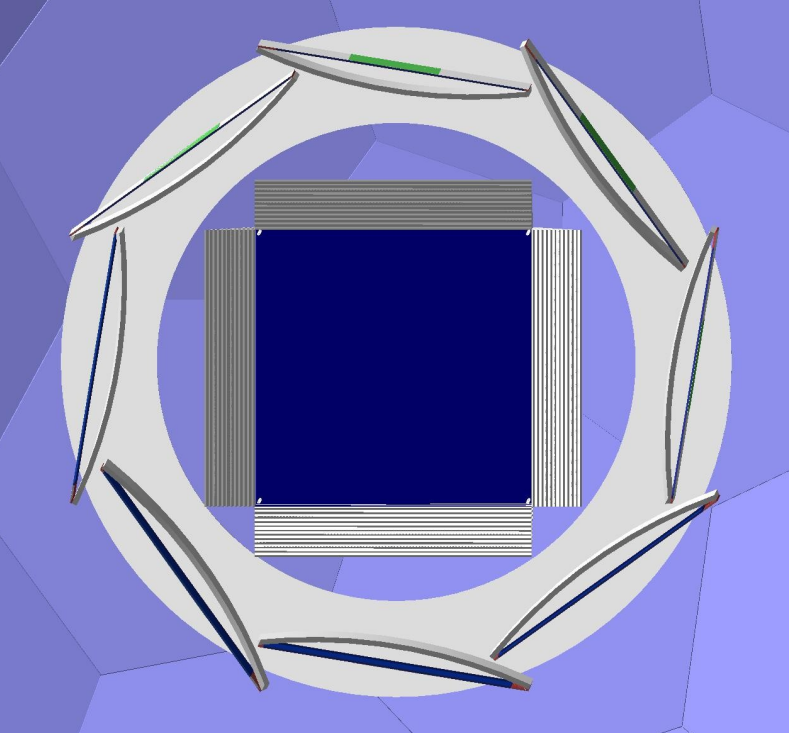
\includegraphics[width=0.55\textwidth]{../resources/figures/chapters/01_introduction/simulated_tracker_2}
  \caption{Example tracker concept used in simulation studies. The tracker
  option is being evaluated as a low-mass detector for positron direction,
  calorimeter matching, and possible trigger information.}
  \label{fig:tracker-simulation-concept}
\end{figure}

The main design question is whether the information gained from a separate
tracker is sufficiently complementary to what can be extracted from the ATAR.
Simulation studies have tested whether tracker hits, possibly combined with
the last ATAR layers, improve trigger efficiency or reduce energy-dependent
trigger bias. In the simplified studies available so far, a low-threshold
calorimeter trigger dominates the combined efficiency
\cite{rohe_track_trigger_2026,schwendimann_spa_tracker_2026}. A tracker may
still be justified if it provides a more robust polar-angle estimate, better
matching to the calorimeter, or cleaner trigger primitives than the ATAR can
provide on its own. Conversely, improved ATAR reconstruction, including
machine-learning approaches that bootstrap information from simulated or
external tracking, may recover much of the same directional information
without requiring a separate tracker. The tracker decision is therefore tied
to ongoing reconstruction, trigger, and detector-optimization studies.

\subsection{Active Target}
\label{subsec:detector-overview-atar}

The active target (ATAR) is the central detector element that makes the
PIONEER strategy qualitatively different from previous \(R_{e/\mu}\)
measurements. It is both the pion stopping target and a high-granularity
silicon detector. Its job is not to replace the calorimeter energy
measurement, but to classify the decay topology in space, time, and deposited
energy. In direct
\(\pi\to e\nu\) decay the target should see a pion stop followed by an
outgoing positron. In the dominant \(\pi\to\mu\to e\) chain it should also see
the short \(\withunit{4.1}{\mega\electronvolt}\) muon track before the Michel
positron. Identifying this extra track is essential because the
\(\pi\to\mu\to e\) chain is roughly four orders of magnitude more common than
the direct electronic decay. Even a small probability for this dominant
normalization channel to be misidentified as a direct pion decay would create
a background comparable to, or larger than, the signal sample.

The baseline ATAR technology is based on low-gain avalanche diodes (LGADs),
with AC-coupled LGADs and related high-fill-factor technologies under study.
An LGAD is a thin silicon sensor with a moderate internal gain layer, allowing
for fast timing. The detector is
designed as a compact silicon stack with
approximately \(\withunit{2}{\centi\meter}\times
\withunit{2}{\centi\meter}\) transverse area and total active thickness of
roughly \(\withunit{6}{\milli\meter}\) along the beam direction
\cite{mazza_high_granularity_atar_2023}. A representative strip design uses
\(\withunit{200}{\micro\meter}\) pitch, alternating strip orientations in
48 successive planes, and thin sensors of order
\(\withunit{120}{\micro\meter}\). With 100 strips per plane, this
representative geometry gives 4800 readout channels. The alternating strip
geometry provides position information while keeping readout electronics
outside the active volume to reduce inactive material in the path of outgoing
positrons
\cite{mazza_lgad_active_target_2022,mazza_high_granularity_atar_2023}.

\begin{figure}[!htbp]
  \centering
  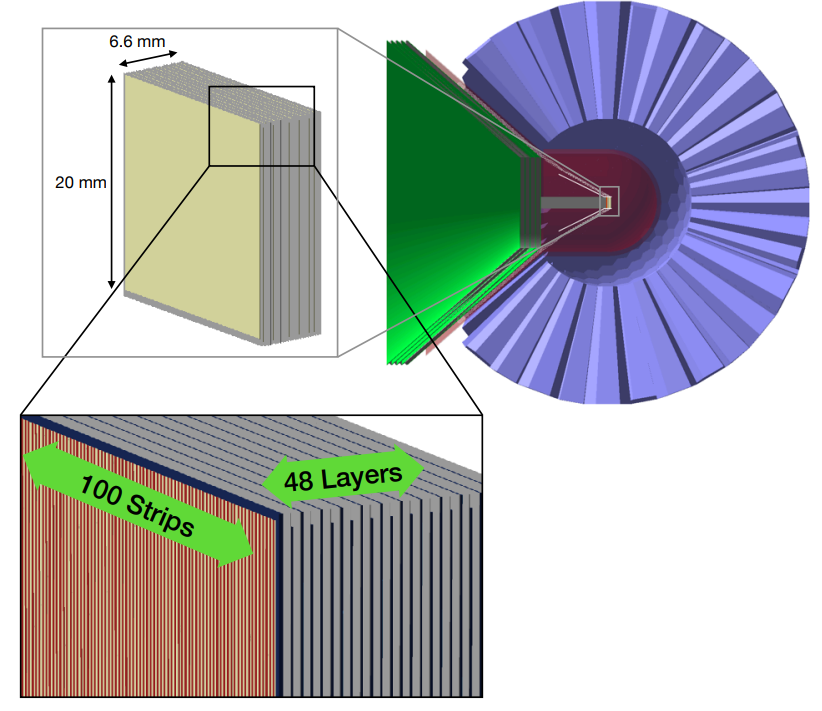
\includegraphics[width=0.52\textwidth]{../resources/figures/chapters/01_introduction/atar_design}
  \caption{Figure 1.10: Schematic ATAR stack concept. 
  Alternating strip orientations provide three-dimensional position reconstruction, precise timing, 
  and energy-deposition measurements while keeping inactive material low.}
  \label{fig:atar-design-overview}
\end{figure}

The performance requirements follow from the physical separation of the pion
and muon decay signatures. A \(\withunit{4.1}{\mega\electronvolt}\) muon from
\(\pi\to\mu\nu\) travels only about \(\withunit{750}{\micro\meter}\) before
stopping, so position resolution at the \(\order{\withunit{100}{\micro\meter}}\)
scale is needed to separate the pion and muon stops. Current ATAR key
performance parameters target single-hit spatial resolution of order
\(\withunit{60}{\micro\meter}\), timing below
\(\withunit{200}{\pico\second}\) per hit, positron energy-deposit resolution
below about \(\withunit{20}{\percent}\), and separation of pulses spaced by
roughly \(\withunit{1.5}{\nano\second}\)
\cite{atar_kpp_2025,mazza_lgad_active_target_2022,mazza_high_granularity_atar_2023}.
The energy-deposit dynamic range is unusually large, spanning positron
signals of order a few tens of \(\keV\) to multi-\(\MeV\) Bragg peaks from
stopping pions and muons.

These requirements drive the ATAR sensor program. The detector must resolve
close-by hits in a high dynamic range environment while keeping inactive
material low enough that it does not degrade the calorimeter measurement.
Material-control targets include only tens of microns of dead material between
active planes and a small amount of silicon and flex material around the ATAR,
because inactive material directly affects the outgoing positron before it
reaches the calorimeter \cite{atar_kpp_2025}. If achieved, the ATAR provides
event-by-event rejection of
\(\pi\to\mu\to e\) backgrounds, identification of pion and muon decays in
flight, pileup rejection, and an in situ handle on the low-energy positron
response tail. These capabilities are the experimental
reason that the detector can aim for a substantially smaller systematic
uncertainty than previous pion-decay measurements
\cite{pioneer_proposal_2022,mazza_high_granularity_atar_2023}. A brief
summary of LGAD sensor technology is given in
\appref{sec:appendix-lgad-technology}.
\FloatBarrier
